\section{Medidas de rendimiento}

Las medidas de rendimiento de una red nos sirven para ver de manera croncreta como se comporto nuestra red, durante el entrenamiento, que fue lo que pudo aprender, que sobre aprendio es decir memorizo, y que aún le cuesta trabajo aprender y por tanto será incapaz de predecir. Se usan las siguientes:

\begin{description}
 \item [Matriz de confusión]: Cuenta los errores, aciertos. Facilita a ver cuando un clasificador está condundiendo clases. Las columnas representan los valores esperados, mientras que las filas los valores de salida. Así que si los valores que no estan en la diagonal de la matriz son cero podemos decir que nuestro modelo aprendio la tarea dada.
 
 \begin{figure}[H]
 \centering
 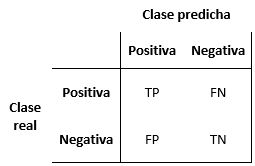
\includegraphics[scale=0.7]{../Figuras/Matriz_confusion_binaria.jpg}
 \caption{Matriz de confunsión para elementos booleanos, Errachete, 17 Diciembre 2019, Wikimedia Commons, \url{https://upload.wikimedia.org/wikipedia/commons/b/b3/Matriz_confusion_binaria.jpg}, CC BY-SA 4.0}
 \label{fig:matrix} 
\end{figure}

 \item [Precisión y recupecación (recall)]: Para saber que tan presisa fue nuestro modelo se usa la equación P, y para saber que tanto se equivoco la ecuación R. Descritas acontinuación, donde \emph{FN} es falso negativo, dio negativo cuando se esperaba positivo, \emph{FP} es falso positivo, dio positivo cuando se esperaba negativo, \emph{VP} es verdadero positivo, dio positivo y se esperaba positivo, y \emph{VN} es verdadero negativo, dio negativo y se esperaba negativo:
    \begin{equation}
        P = \dfrac{VP}{VP+FN} 
    \end{equation}
    \begin{equation}
        R = \dfrac{VP}{VP+FP} 
    \end{equation}
    
    \begin{itemize}
     \item Cuando el modelo detecta los ejemplares pero los incluye en otras clases también: \emph{P} es bajo y \emph{R} es alto. 
     \item Cuando el modelo no detectó bien los ejemplares pero tampoco los incluyo en otras clases: \emph{P} es alto y \emph{R} es bajo. 
     \item Cuando el modelo detecta los ejemplares y no los incluye en tras clases:\emph{P} y \emph{R} es alto. 
     \item Cuando el modelo no detecta los ejemplares:\emph{P} y \emph{R} es bajo. 
     \end{itemize}

 \item [Exactitud (accurrancy) y f (f score)]: La accurrancy es para ver que tan cerca estuvimos de identificar los valores esperados (no se recomienda usar si tienes clases desbalancedas, es decir, muchos elementos de una clase y poco de otra pues nos puede fallar totalmente con las clases pequeñas y aún así su valor sería alto). La \emph{f} se utiliza para combinar las medidas de precision y recall en un sólo valor. Es práctico porque hace más fácil el poder comparar el rendimiento combinado de la precisión y la recall entre varias soluciones. Se dan las ecuaciones acontinuación:
    
    \begin{equation}
     A = \dfrac{VP+VN}{VP + VN + FP + FN} = \dfrac{VP+VN}{Todos los valores clasificados}     
    \end{equation}

    \begin{equation}
     F = \dfrac{2}{\dfrac{1}{P} +\dfrac{1}{R} }= 2 \dfrac{P * R}{P + R}
    \end{equation}

\end{description}

